\documentclass[9pt,twocolumn,twoside]{styles/osajnl}
\usepackage{fancyvrb}
\journal{i524} 

\title{Apache Drill}

\author[1,*, +]{Yatin Sharma}

\affil[1]{School of Informatics and Computing, Bloomington, IN 47408, U.S.A.}

\affil[*]{Corresponding authors: yatins@indiana.edu}

\affil[+]{HID - S17-IR-3000}

\dates{Paper-001, \today}

\ociscodes{Apache, Drill, DrillBit, NoSQL, Query}

% replace this with your url in github/gitlab
\doi{\url{https://github.com/yatinsharma7/sp17-i524/tree/master/paper1/S17-IO-3000/report.pdf}}


\begin{abstract}
	Apache Drill is a distributed SQL engine designed to enable users to explore and analyze data stored in non-relational datastores. It enables users to query the data using standard SQL and BI tools without having to create schemas or transform data. 
	\newline
\end{abstract}

\setboolean{displaycopyright}{true}

\begin{document}

\maketitle

\section{Introduction}
Apache Drill\cite{Drill}, inspired by Google's Dremel System, is industry's first schema-free distributed SQL Engine which allows us to write SQL queries without having the need to define and maintain schemas or transform data(ETL). It automatically understands the structure of the data. It can integrate and combine from several data sources like hive, hbase, mongodb, etc in a single query and export the data to any of the reporting tools like tableau, Excel, etc. It can help to save a lot time in data processing, which earlier consumed majority of projects time.

\section{Benefits}
Apache Drill allows us to conduct research on datasets without having to be an expert in everything.It allows to couple various datasets with NO SQL systems and provide direct access to keys of data which can then be used to query the data using Apache Drill whether it is stored in a file or NO SQL database.
From a security perspective, Drill allows to create views for higher level access on the original data and give permission to others on these views.You don't have to worry about creating security database, you can simply create a view and apply filesystem security to this view based upon your needs. Drill currently supports 3 layers of impersonation.

\section{Architecture}
Drillbit \cite{Drillbit} is apache drill's daemon which runs on each node in the cluster. It uses ZooKeeper for all sort of communication in the clusters. ZooKeeper is basically responsible for cluster combination, cluster membership, leadership selection, etc. So, when ever we fire a query, the ZooKeeper finds the Drillbit instance, also called foreman, which will eventually do the parsing, optimization, execution and data aggregation. All of this takes fraction of seconds to execute. Just like Mapreduce, It is all about data locality in which there is no need to change data over the network and instead bring code to the data. Everything in Drill is done in a distributed manner.

\subsection{Query Execution Flow}
The SQL query comes in from the client, which could be jdbc, odbc, etc, is accepted by a drillbit. This drillbit that accepts this acts as a foreman for this particular request. As a client application you can either submit to a drillbit or talk to the zookeeper which in turn will route this to an available drillbit. Once the query is received, it parses the query and tries to figure out the most optimal way to execute this query. Drill allows to do a variety of rule based as well as cost based optimization in addition to being aware of data locality while doing the query planning. Once the query plan is determined, Drill splits the query plan into a number of pieces called 'Query Plan Fragments'. The coordinated drillbit talks to the ZooKeeper and finds out what are the other drillbits that are available in the cluster. It then gets the location of the data and combines this information to determine the drillbits that can handle this Query Plan Fragments. It distributes the work to other drillbits in the cluster. Each Drillbit then does its own processing of the Query Plan Fragment and returns the result to the original drillbit which then combines and returns the result to the client. As shown in the diagram below, Each of the drillbit, during the execution, would be interacting with the underlying Storage System like DFS, Hbase, MongoDB, etc.

\begin{figure}[htbp]
	\centering
	\fbox{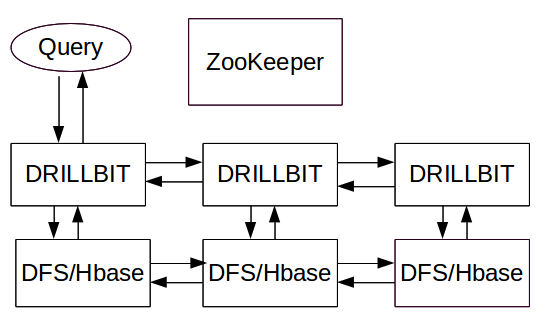
\includegraphics[width=\linewidth]{images/Architecture.png}}
	\caption{Query Execution Workflow.}
	\label{fig:Drill-arch}
\end{figure}

Important thing to notice here is that each of the Drillbits are equal and there is no Master-Slave concept. So, the request from the client can go to any of of the drillbit depending upon its availability. It is also a completely scale-out architecture that allows us to add in more drillbits as and when required\cite{Query-Execution}.

\subsection{Execution Architecture Elements}
\subsection{Columnar Execution}
Drill is Columnar in storage as well as memory. It basically means that it does not have to materialize the data into row format and can perform all SQL operations like join, sorting, etc directly on columnar data  without having to change the data. The benefit of this is that it not only boosts the performance but also saves the memory footprint that Drill has to occupy during query execution.

\subsection{Vectorized Processing}
Instead of working on single records at any given time, Drill allows CPU to work on what is called Vector, which is basically and array of values from set of records in table. So, Drill works on more than one record at a time.

\subsection*{Optimistic/In-Memory}
Drill is very optimistic in the sense it assumes that the chances of failure like hardware or node failure is very uncommon during the short execution of the query.So, it tries to execute as much as possible in memory without writing anything to disk for checkpoint and recovery purposes. Drill uses the traditional Pipe-line execution model in which all the tasks are executed in parallel and in different stages in different parts of the cluster.This enables Drill to achieve high speed performance in seconds.

\subsection{Datastores Support}
Drill is primarily build for non-relation datastores like Hadoop, NoSQL, and cloud storage.
Currently following datastores are supported:

\begin{itemize}
	\item \textbf{Hadoop}: All Hadoop distributions (HDFS API 2.3+), including Apache Hadoop, MapR, CDH and Amazon EMRfor Data Ingestion
	\item \textbf{NoSQL}: MongoDB, HBase
	\item \textbf{Cloud storage}: Amazon S3, Google Cloud Storage, Azure Blog Storage, Swift

\end{itemize}

\subsection{Client Support}
Drill currently supports following clients:

\begin{itemize}
	\item \textbf{BI tools} via the ODBC and JDBC drivers (eg, Tableau, Excel, MicroStrategy, Spotfire, QlikView, Business Objects)
	\item \textbf{Custom applications} via the REST API
	\item \textbf{Java and C applications} via the dedicated Java and C libraries
	
\end{itemize}

\section{Drill vs. Hive}
Hive is a typical batch processing framework best suitable for long-running jobs, Drill 
on the other hand is suitable for short-running jobs like data exploration and BI.
Moreover, unlike Hive, Drill is not limited to Hadoop. For example, it can query NoSQL databases (eg, MongoDB, HBase) and cloud storage (eg, Amazon S3, Google Cloud Storage, Azure Blob Storage, Swift).

\section{Getting started}
It only takes a few minutes to install Drill and there are several Tutorial \cite{Tutorial} available online to help us get started.

\section{Conclusion}
Drill provides a single SQL interface for self service data exploration for structured and semi-structured data Source without any IT intervention and is extremely easy to use. Drill also allows us to use familiar BI tools like tableau and Excel for data exploration without time consuming and expensive programing and data definition.The resulting self service access to data allows data analysis and reduce time to value to a large extent..

\section*{Acknowledgements}

The author thanks Prof. Gregor von Laszewski for his technical guidance.

% Bibliography

\bibliography{references}

\end{document}
